\documentclass[12pt,a4paper]{article}
\usepackage{bold-extra}
\usepackage{appendix}
\usepackage{amsfonts,amsmath,amssymb}
\usepackage{enumerate}
\usepackage{float}
\usepackage{geometry}
\usepackage{graphicx}
\usepackage{latexsym}
\usepackage{listings}
\usepackage{multicol,multirow}
\usepackage{subfigure}
\usepackage{tabularx}
\usepackage{ulem}
\usepackage{tikz}
\usetikzlibrary{angles,quotes}
\usepackage{verbatim}
\usepackage{xcolor}
\geometry{a4paper,left=1in,right=1in,top=1in,bottom=1in}
\begin{document}
\centerline{\Huge{{\textbf{PHYSICS II\ \ Problem Set 6}}}}
\vspace{0.5cm}
\leftline{\large{Name: Haotian Fu}}
\rightline{\large{Student ID: 520021910012}}

\section*{\large \textbf{Problem 1}}~{\textbf{Solution}}
    \par We may discuss the electric force and magnetic force separately.
    \par For the electric force
    \begin{equation}
        ma_E = -qE_0
        \label{eq:p1-electric}
    \end{equation}
    where $a_E$ is the translational acceleration along -$x$-axis.
    \par Hence the change of velocity caused by electric field is
    \begin{equation}
        v_E(t) = \left( -\frac{qE_0}{m}t, 0, 0 \right)
        \label{eq:p1-Ve}
    \end{equation}
    \par For the magnetic force
    \begin{equation}
        qv\times B = m\omega^2 R
        \label{eq:p1-magnetic}
    \end{equation}
    where $R$ is the radius of circular motion.
    \par Hence the change of velocity caused by magnetic field is
    \begin{equation}
        v_B(t) = \left( v_{y_0}\cos\omega t, v_{y_0}\sin\omega t \right)
        \label{eq:p1-Vb}
    \end{equation}
    where $\omega = \frac{B_0q}{m}$
    \par Hence the velocity of the particle is
    \begin{equation}
        v(t) = v_1(t) + v_2(t) = \left( v_{x_0}-\frac{qE_0}{m}t, v_{y_0}\cos\frac{B_0q}{m}t, v_{y_0}\sin\frac{B_0q}{m}t \right)
        \label{eq:p1-V}
    \end{equation}
    Integrate Eq.(\ref{eq:p1-V})
    \begin{equation}
        x(t) = \int_{x(0)}^{x(t)} v(t)dt = \left( v_{x_0}t-\frac{qE_0}{2m}t^2, \frac{mv_{y_0}}{B_0q}\sin\frac{B_0q}{m}t, -\frac{mv_{y_0}}{B_0q}\cos\omega t \right)
        \label{eq:p1-x}
    \end{equation}
    

\section*{\large \textbf{Problem 2}}~{\textbf{Solution}}
    \begin{enumerate}
        \item \begin{align}
                I = JA = Jwh \\ 
                F = I\textit{l} \times B \\ 
                \Delta p = \frac{F}{wh}
            \end{align}
            Hence
            \begin{align}
                \Delta p = J\textit{l}B
            \end{align}
        \item Derived from (a)
            \begin{align*}
                J = \frac{\Delta p}{Bl}
            \end{align*}
            Plug in the data 
            \begin{align*}
                J = \frac{101.325\times 10^3}{2.2\times 35\times 10^{-3}} = 1.3\times 10^6\ [A/m^2]
            \end{align*}
    \end{enumerate}


\section*{\large \textbf{Problem 3}}~{\textbf{Solution}}
    Differential equation 
    \begin{equation}
        dF = Id\textit{l}\times B
    \end{equation}
    Hence
    \begin{equation}
        F = \int\limits_{\text{plane wire}} Id\textit{l}\times B = Iw\times B
    \end{equation}
    Namely, as for the magnitude
    \begin{equation}
        F = IBw
    \end{equation}
    where the direction of the force is related to the direction of current. If the current is clockwise, the force points upwards while if the current is counter-clockwise, the force points downwards.


\section*{\large \textbf{Problem 4}}~{\textbf{Solution}}
    \begin{enumerate}[(a)]
        \item \begin{figure}[!htbp]
                \begin{small}
                    \begin{center}
                        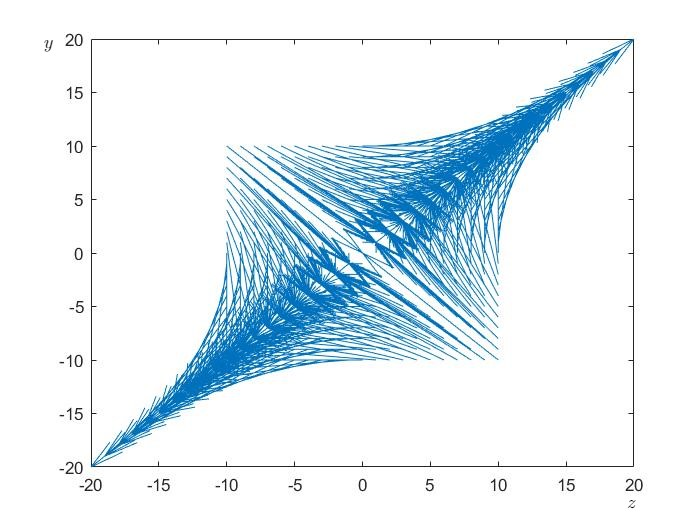
\includegraphics[width=0.6\textwidth]{p4-a.jpg}
                    \end{center}
                    \caption{The magnetic field lines in the $yz$-plane}
                \end{small}
            \end{figure}
        \item \begin{equation}
                dF = Id\textit{l}B
            \end{equation}
            \par For the lower wire, since both $y$ and $z$ are equal to zero, there is no magnetic field, thus $F=0$.
            \par For the left wire, $z=0$, hence
            \begin{equation}
                F = I\frac{B_0}{L}\int_0^L y\,dy = \frac{ILB_0}{2}
            \end{equation}
            \par For the upper wire, $z=0, y\equiv L$, hence
            \begin{equation}
                F = ILB_0
            \end{equation}
            \par For the right wire, $z=0$, analogous to the left wire 
            \begin{equation}
                F = -\frac{ILB_0}{2}
            \end{equation}
        \item Add all the force appearing in (b)
            \begin{equation}
                F_{\text{total}} = ILB_0 = \left(0,ILB_0,0\right)
            \end{equation}
    \end{enumerate}


\section*{\large \textbf{Problem 5}}~{\textbf{Solution}}
    \begin{enumerate}[(a)]
        \item \begin{equation}
                F = \int\limits_{\Sigma} Id\textit{l}B = \oint Id\textit{l}B = IB \oint d\textit{l} = 0
            \end{equation}
        \item 
    \end{enumerate}
    


\section*{\large \textbf{Problem 6}}~{\textbf{Solution}}
    \begin{enumerate}[(a)]
        \item \begin{equation}
                T = \frac{2\pi R}{v} = \frac{2\pi\times 5.3\times 10^{-11}}{2.2\times 10^6} = 1.5\times 10^{-16}\ [s]
            \end{equation}
        \item \begin{equation}
                I = \frac{e}{T} = 1.1\times 10^{-3}\ [A] 
            \end{equation}
        \item \begin{equation}
                \mu = (IA)\hat{n} = I\pi R^2 = 9.7\times 10^{-24}\hat{n}\ [Am^2]
            \end{equation}        
    \end{enumerate}
    
    
\end{document}